% chapter literature review

\section{Grid Computing}
Grid computing \cite{li2005grid} is the technology innovation in high performance computing. A large number of scientists work on the operations of this huge co-operative project of EU. Monitoring \& information architecture \cite{fisher2002datagrid} has been standardized in the initial state of that project, to succeed in building a large-scale production grid of 150.000 cores. Use of grid computing nowadays takes place in academic and research environments. Also, applications in industry-based needs such as promising Power Grid control \cite{Taylor2006} are emerging.

Grid computing may be the infrastructure over which Cloud Computing may reside. Cloud computing promise that it will change how services are developed, deployed and managed. The elastic demands of education and research community is a good place where cloud computing may be developed. Many datacenters all over Europe which are currently serving grid computing infrastructure for \ac{LHC}, could later share the resources to help some other big academic projects scale up as needed.

\section{Resource Brokers}
Resource Brokers \cite{Kertesz06ataxonomy} were developed to manage the workload on Computer elements and Resource elements. Globus is a non-service based RB, and gLite RB which is service based. A \ac{WMS} exists in gLite to do the distribution and management of the Computing and Storage oriented tasks.

The use of information system is based on the equivalent middleware that resource brokers rely on. From resource broker's point of view, the relevant information is the data store and query. There are two main categories of information systems in middlewares. The Directory-based and the Service-based. They are used for resource mapping by the brokers when they access the resource data.

\begin{figure}[h]
\begin{center}
% Set the overall layout of the tree
\tikzstyle{level 1}=[level distance=3.5cm, sibling distance=3.5cm]
\tikzstyle{level 2}=[level distance=3.5cm, sibling distance=2cm]

% Define styles for bags and leafs
\tikzstyle{bag} = [text width=4em, text centered, circle, thick]
\tikzstyle{end} = [circle, minimum width=3pt,fill, inner sep=0pt]

% The sloped option gives rotated edge labels. Personally
% I find sloped labels a bit difficult to read. Remove the sloped options
% to get horizontal labels. 
\begin{tikzpicture}[grow=right,sloped]
\node[bag] {Data Store and Query}
    child {
        node[bag] {WSRF}        
            child {
                node[end, label=right:
                    {MDS4}] {}
                edge from parent
                node[above] {}
                node[below]  {}
            }
            child {
                node[end, label=right:
                    {MDS3}] {}
                edge from parent
                node[above] {}
                node[below]  {}
            }
            edge from parent 
            node[above] {}
            node[below]  {}
    }
    child {
        node[bag] {LDAP}        
        child {
                node[end, label=right:
                    {MDS2}] {}
                edge from parent
                node[above] {}
                node[below]  {}
            }
            child {
                node[end, label=right:
                    {BDII}] {}
                edge from parent
                node[above] {}
                node[below]  {}
            }
        edge from parent         
            node[above] {}
            node[below]  {}
    };
\end{tikzpicture}

\caption{Grid Resource Brokers grouped by Information Systems\cite{Kertesz06ataxonomy}}
\end{center}
\end{figure}

\subsection{Globus}

Globus Toolkit is an open source toolkit used to build grids. It provides standards such as \ac{OGSA}, \ac{OGSI}, \ac{WSRF} and \ac{GSI}, and the implementations of \ac{OGF} protocols such as \ac{MDS} and \ac{GRAM}.

\begin{figure}[htb]
\centering
 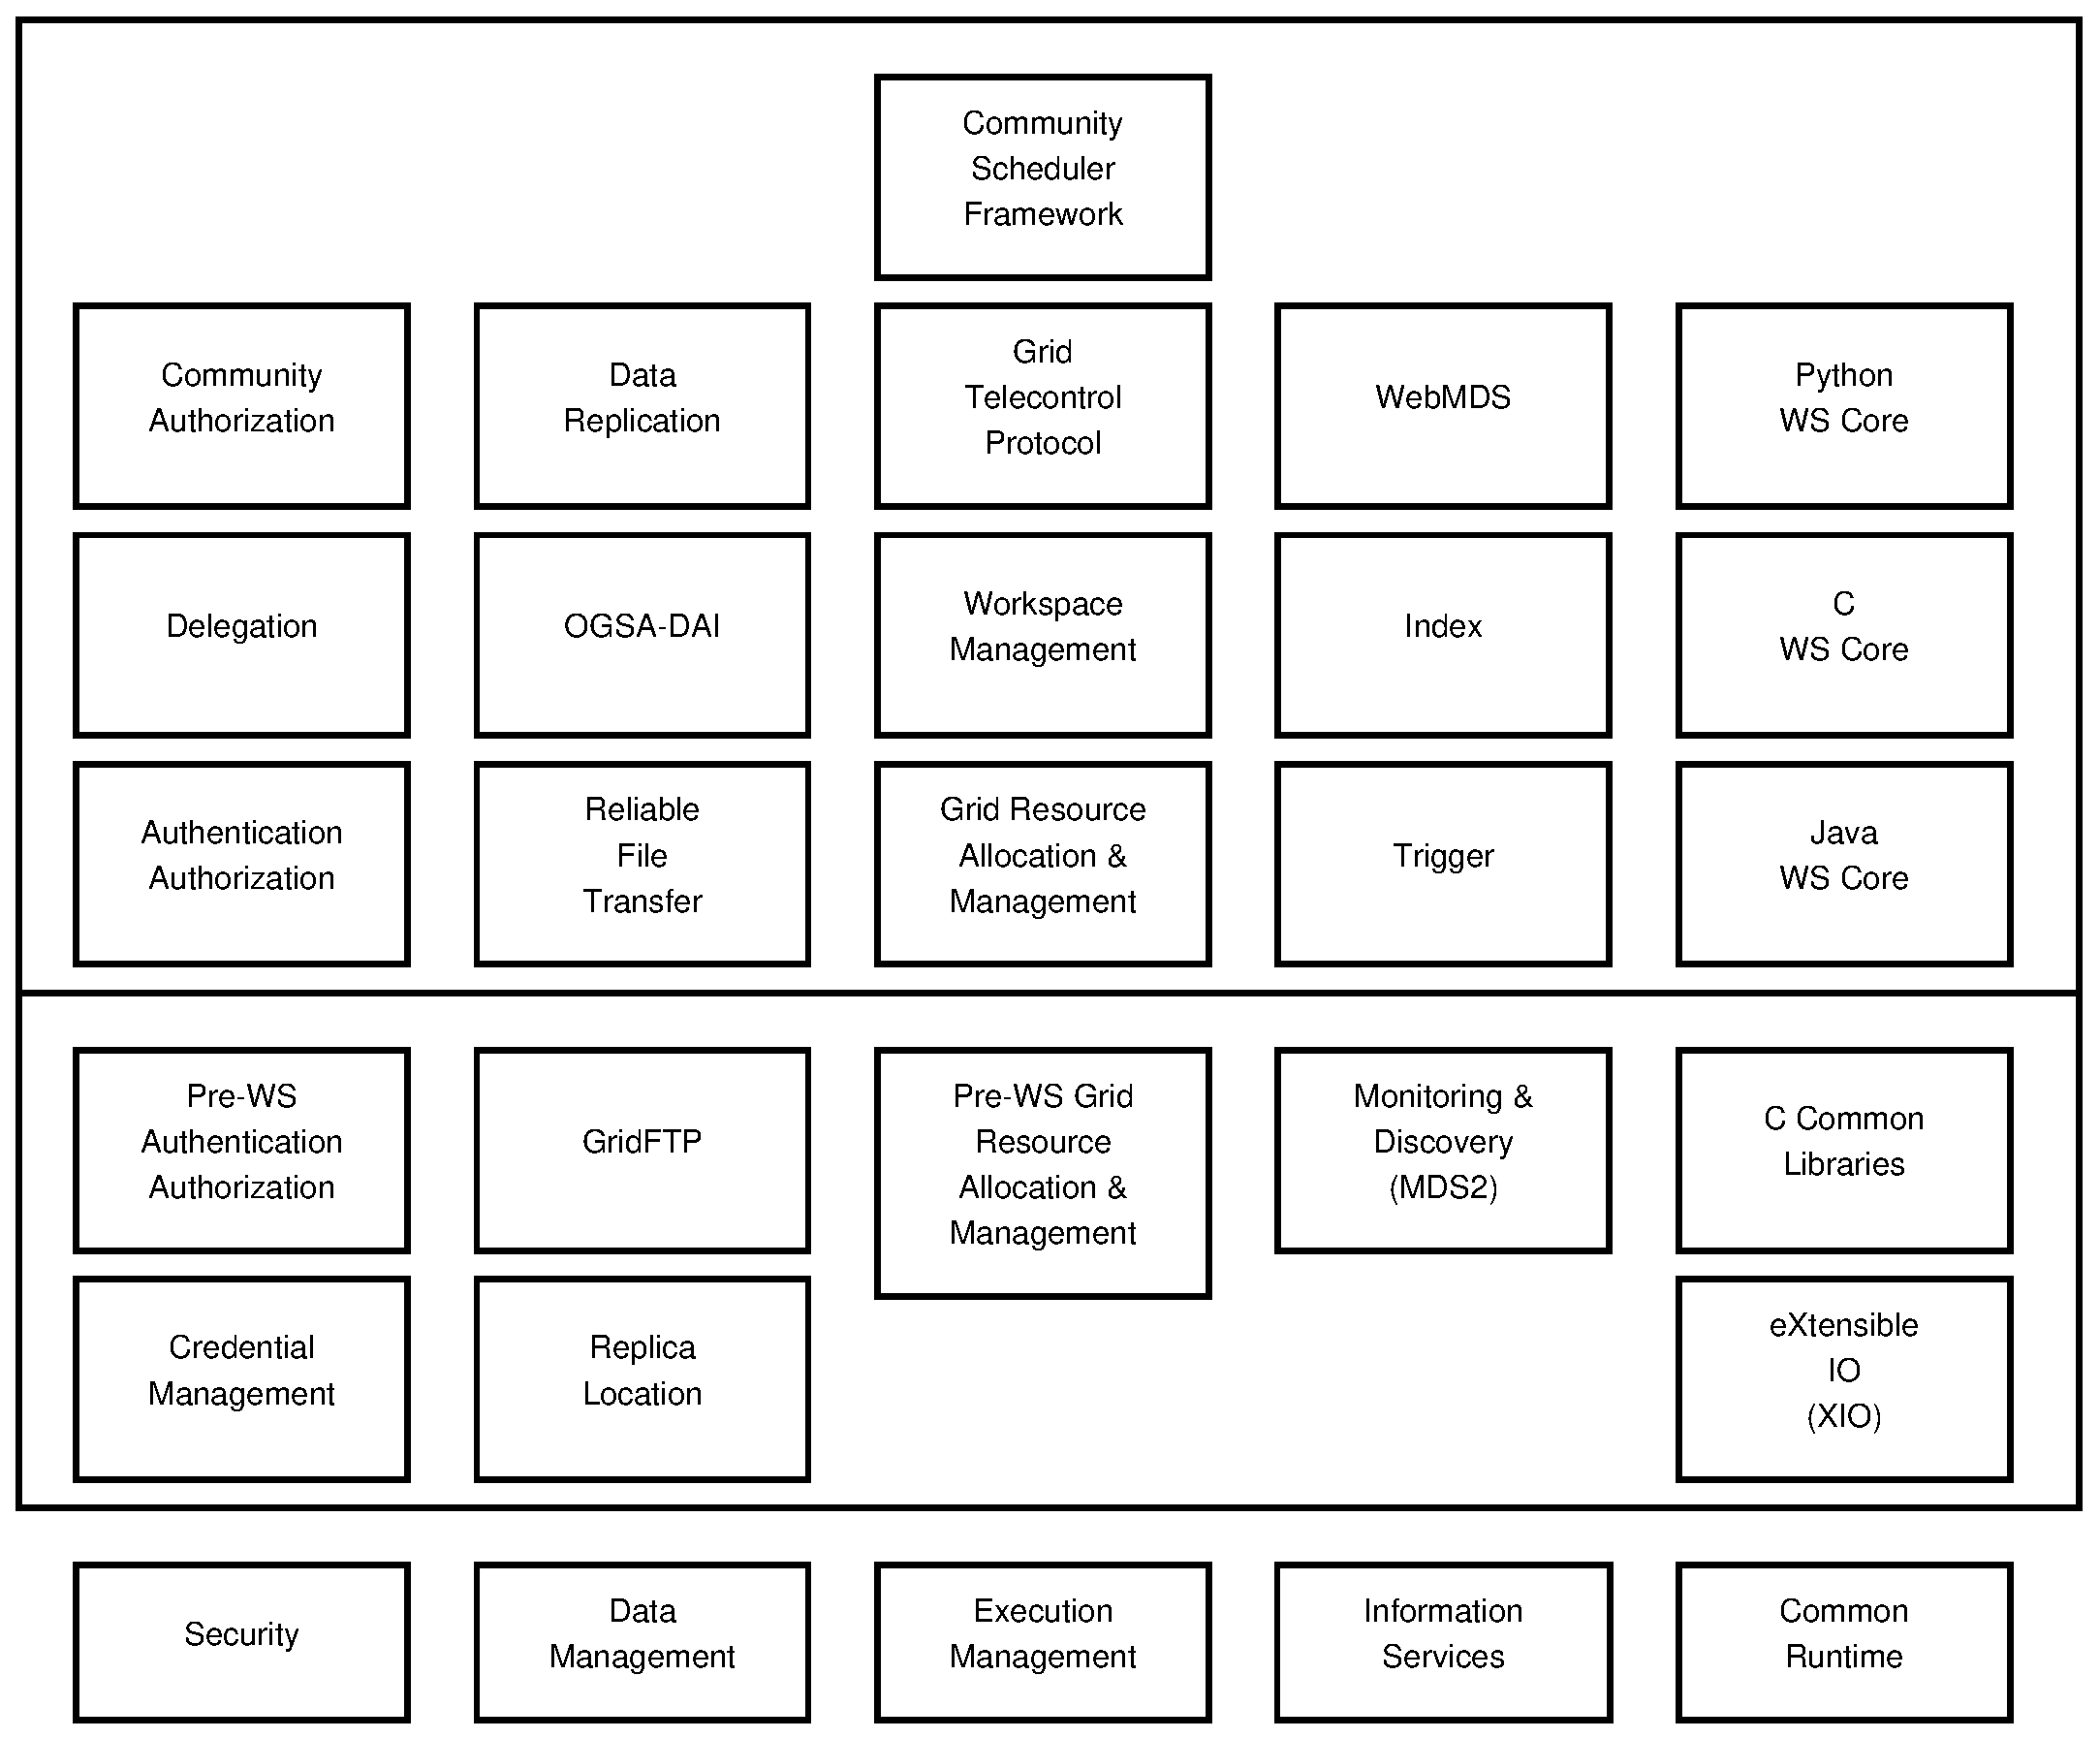
\includegraphics[width=130mm]{images/globus.eps}
\caption{\ac{GT4}}
\label{figure:globus}
\end{figure}

\ac{MDS} is part of Globus Toolkit, and provides the information for the availability and status of grid resources. As a suite of Web Services, it offers a set of components that help to the discovery and monitoring of the resources that are available to a \ac{VO}.

\subsection{gLite}

gLite is a middleware which was created to be used in the operation of the experiment \ac{LHC} in CERN. The user community is grouped in \acp{VO} and the security model is \ac{GSI}. A grid using gLite consists of \ac{UI}, \ac{CE}, \ac{SE}, \ac{WMS} and the Information System.

\begin{figure}[htb]
\centering
 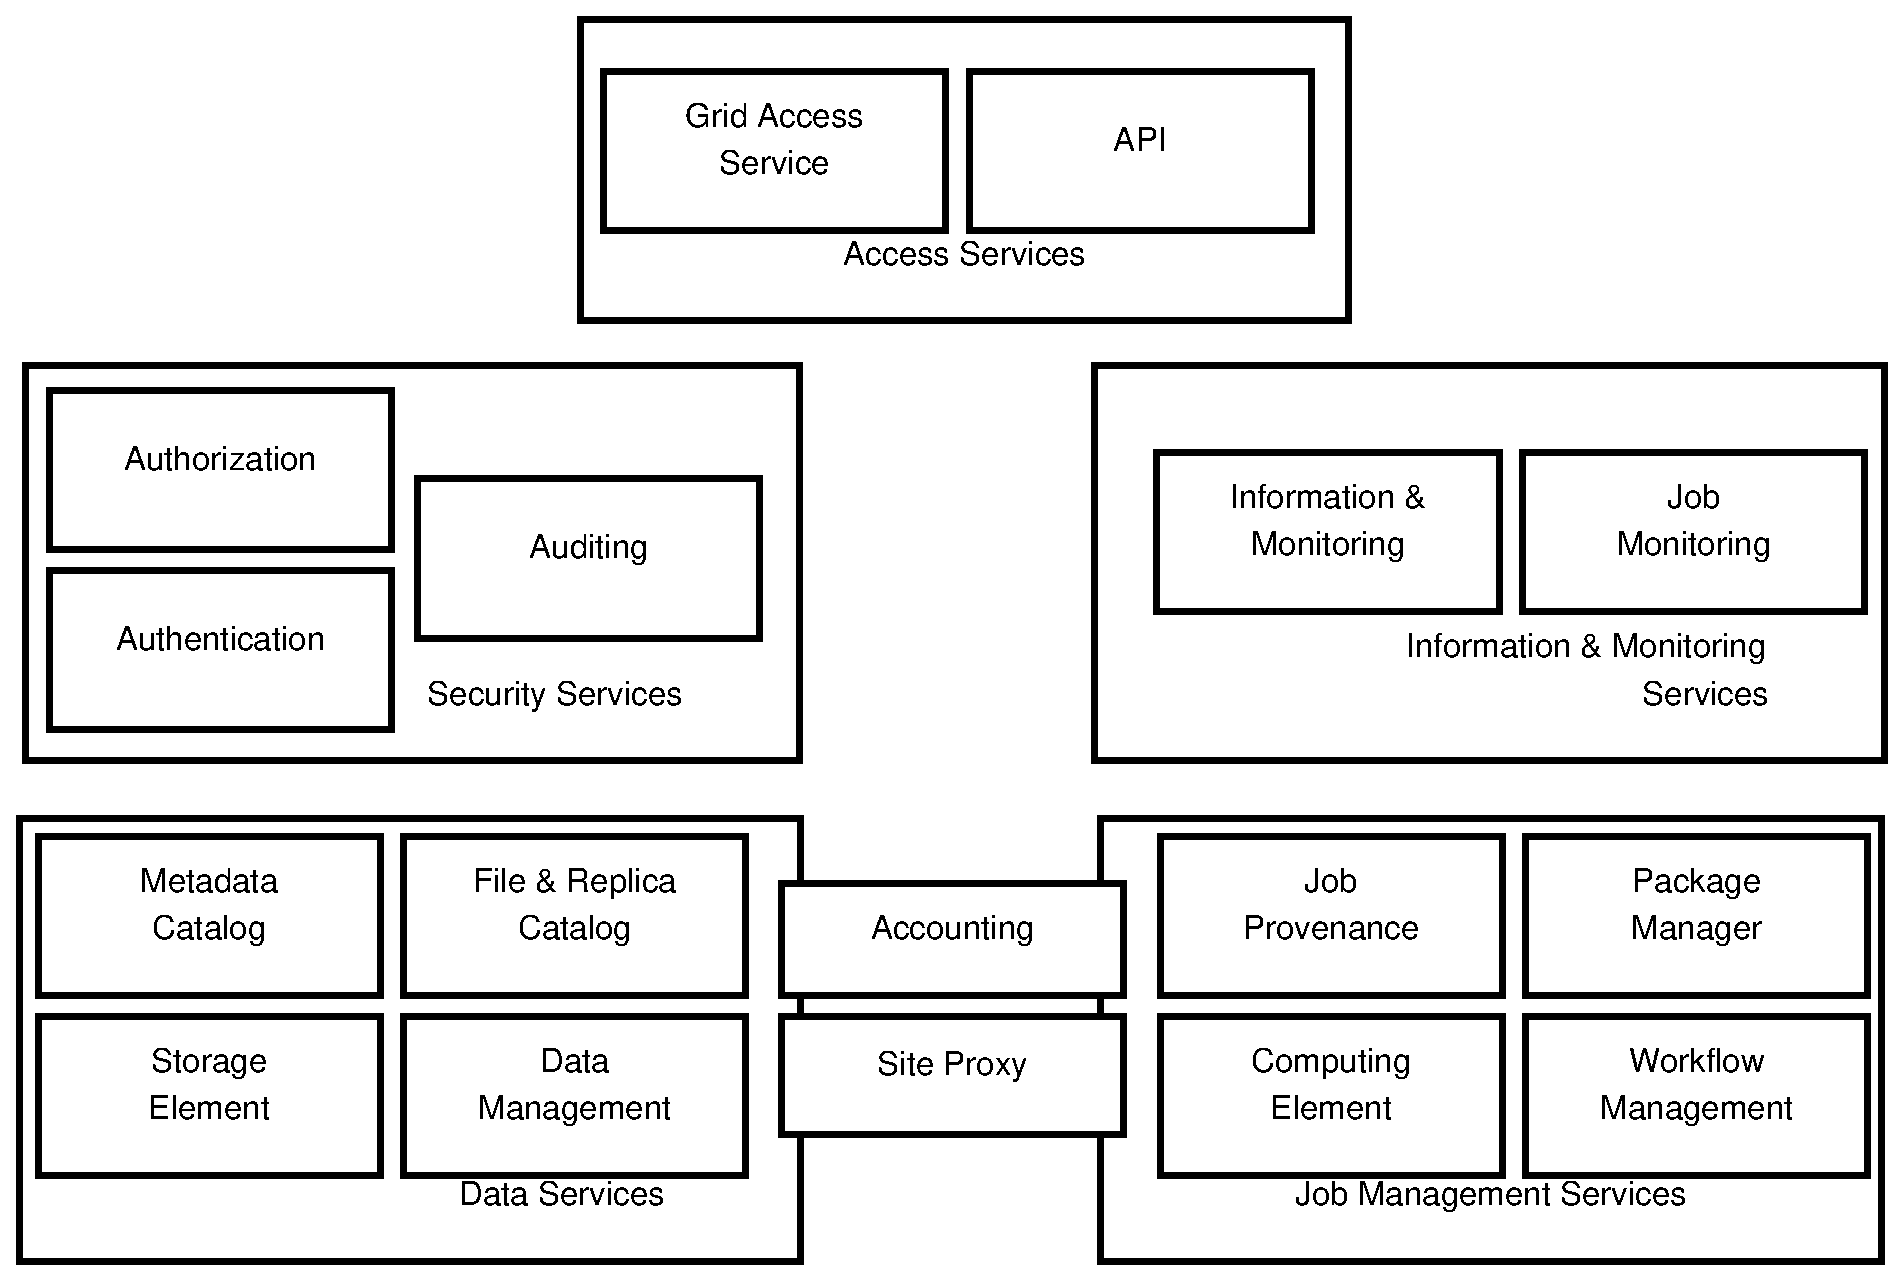
\includegraphics[width=130mm]{images/glite.eps}
\caption{gLite architecture}
\label{figure:glite}
\end{figure}

The information service in version $3.1$ of gLite is almost similar to \ac{MDS} of Globus middleware. The only difference is that the \ac{GRIS} and \ac{GIIS} are provided by \ac{BDII} (see Section \nameref{subsec:BDII}) which is an LDAP based service.

\section{Information Services}
A \ac{GMA} \cite{tierney2002grid} was proposed in early 2000's. Information systems were developed to create repositories of information needed to be stored for monitoring and statistical reporting reasons. Such an organized system later was specified by the \ac{ATP} definition. The largest world grids adopt that model, forming \ac{OIM} in \ac{OSG} (USA) and \ac{GOCDB} as that information base in \ac{EGEE} (Europe). Message Bus was also defined as a mean to transfer the underlying data, and many tools came up such as Gstat, \ac{GOCDB} and \ac{BDII} with Glue specification. Grid performance monitoring and keeping of such an information system has also impact in the performance of the system itself \cite{zhang2003performance}, so various methods were developed to give the solution to the scaling and performance problem, such as \ac{MDS}2 (\ac{GIIS} \& \ac{GRIS}), \ac{GMA} and \ac{R-GMA} \cite{wilson2004information}, which offers relational environment \cite{fisher2001relational}, has experience on production systems \cite{byrom-production} and scales to reach huge needs such as \ac{CMS} project \cite{Bonacorsi2004,Byrom}.

\subsection{\ac{MDS}}
Monitoring and Discovery Services is about collecting, distributing, indexing and archiving information of the status of resources, services and configurations. The collected information is used to detect new services and resources, or to monitor the state of a system.

Globus Toolkit was using LDAP-based implementation for its information system since its early versions, back in 1998 \cite{von1998usage}. \ac{MDS}2 in Globus Toolkit fully implemented referral with a combined \ac{GRIS} and \ac{GIIS}, using mds-vo-name=local to refer to the \ac{GRIS} and all other strings to refer to a \ac{GIIS}. It was widely accepted as a standard implementation of a grid information system \cite{945188}, with good scalability and performance \cite{zhang2004performance}.


\ac{MDS} 4 consists of the \ac{WSRF} and a web service data browser, WebMDS. The \ac{WSRF} Aggregator Framework includes:

\begin{enumerate}
  \item MDS-Index, which provides a collection of services monitoring information and an interface to query such information.
  \item MDS-Trigger, which provides a mechanism to take action on collected information.
  \item MDS-Archive, is planned for future release of MDS, to provide access to archived data of monitoring information.
\end{enumerate}

External software components that are used to collect information (such as Ganglia)\cite{gangliaWSRF} are called Information Providers.


\subsection{Glue}
As long as Information Services are used to connect different infrastructures, the schema of its structure had to be standardized. To interoperate EU and USA grids, DataTAG developed the \ac{GLUE} schema implementation. \ac{GLUE} specification quickly was adopted by the communities and currently its recommended LDAP \ac{DIT} is specified in \ac{GLUE} specification v.$2.0$ from GLUE Working Group of \ac{OSG}.

Many objectclasses of the Glue schema define a \ac{CE}, a \ac{SE}, etc. As seen in Figure \ref{figure:gluece_ext} in later chapter, performance monitoring attributes such as processor load, are defined in objectclasses that extend Computer Element objectclass.

\subsection{BDII}\label{subsec:BDII}
\ac{BDII} is used by gLite as the Information Index Service of the \ac{LHC} experiment. It is LDAP based and may be at top-level or site-level. The \ac{GIIS} has been replaced by site \ac{BDII}, which is fundamental for a site in order to be visible in the grid.

Top-level \ac{BDII} contains aggregated information about the sites and the services they provide. Site \ac{BDII} collects the information from its \acp{CE}, \acp{SE}, etc. It also collects information for each configured service that is installed on the site.

Information about the status of a service and its parameters is pushed on \ac{BDII} using external processes. An information provider is also used (such as in \ac{WSRF}) to describe the service attributes using the \ac{GLUE} schema.

\begin{figure}[htb]
\centering
 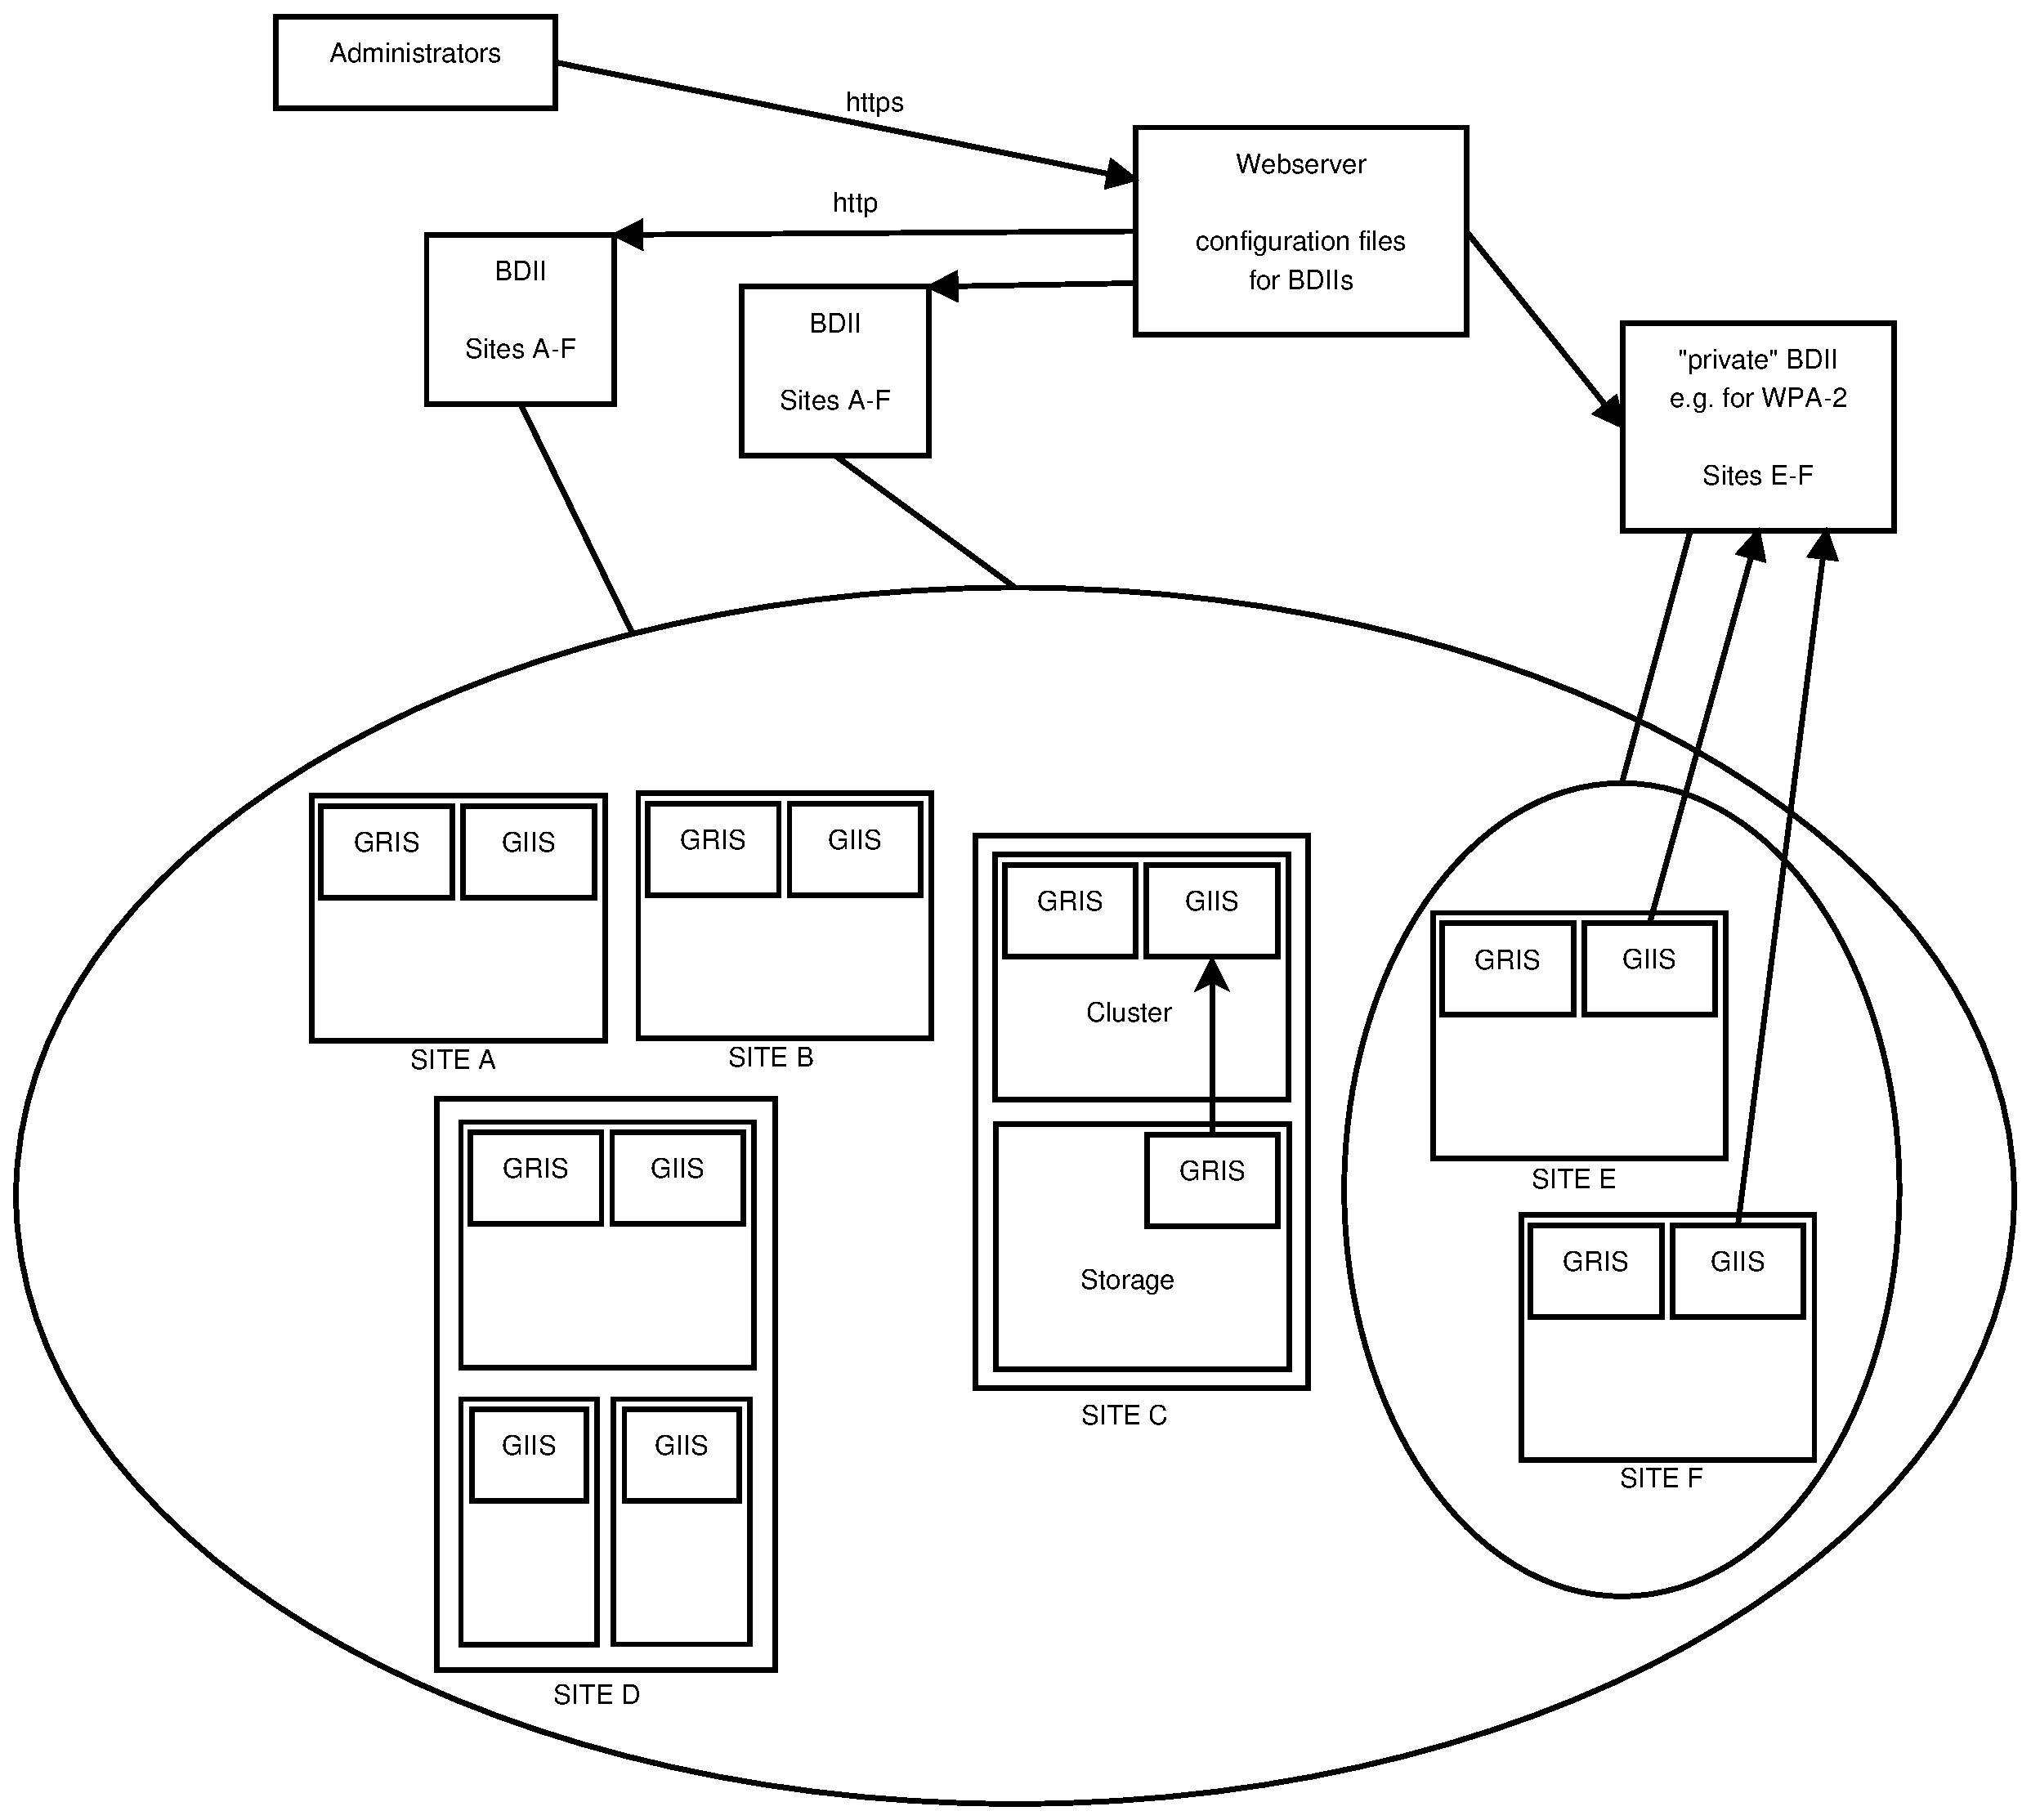
\includegraphics[width=130mm]{images/bdii.eps}
\caption{\ac{BDII}}
\label{figure:bdii}
\end{figure}

\section{Performance Monitoring}
After \ac{EGEE}, the \ac{EGI} was formed to lead in the explosion of the european grid computing community to regional initiatives. Performance and availability monitoring tools and views also follow that format. The result is the phase out of \ac{SAM} \cite{egee3dsa122} and the adoption of Nagios as the tool for regional grid performance monitoring.

A taxonomy effort has been made \cite{gerndt2004performance} to present the differences of performance monitoring systems of the grid, and later a more general \cite{zanikolas2007importance} taxonomy paper was published to give a more general view of these tools. GridICE was generally used to aggregate the performance metrics of \acp{ROC} in high level reports \cite{andreozzi2005gridice}. Later GridICE was left, as \ac{SAM} did, to meet the milestone of \ac{EGI} to have a regional monitoring tool (Nagios) to report the reliability of the joined sites and report the values for \ac{SLA} reasons.

Grid performance can be also measured using benchmark tools in different levels of the grid architecture, using the micro-benchmarks at the Worker Node level, the Site (\ac{CE}) level and the Grid \ac{VO} level. Different metrics and benchmarks exist, such as the measurement of the performance of CPUs in {\bf MIPS using EPWhetstone} and the evaluation of the performance of a CPU in {\bf FLOP/s and MB/s using BlasBench}. GridBench \cite{gridbench} provides a framework to collect those metrics using its own description language, \ac{GBDL}.

GcpSensor \cite{gcpsensor} introduce a new performance metric called WMFLOPS. It uses \ac{PAPI} \cite{papi} to access the hardware performance counters. For data distribution it uses \ac{MDS} information system which provides dynamic metrics for CPU load average for 1, 5 and 15 minutes load.

Linux kernel provides built-in functions to monitor system performance using a metric called $load$. It is a method of individual system performance reporting based on the counter of processes running or waiting in the queue of the Operating System scheduler. This differs from the percentage load average report.

This project focuses on mathematically compute of the performance of a grid based on the metrics that are taken at the Worker Node level.

\subsection{Ganglia}

Ganglia is a monitoring tool which provides a complete real time monitoring environment. It is used by both academia and industry community to monitor large installations of clusters and grids. Any number of host metrics may be monitored in real time using the monitoring core, a multithreaded daemon called Gmond. It runs on every host that is in scope of monitoring. Its four main responsibilities are:

\begin{enumerate}
\item Monitor the changes that happen in the host state
\item Multicast over the network, the changes that has been made
\item Listen to network for changes that other ganglia nodes are multicasting and
\item Answer the status of the whole cluster to specific requests, using XML.
\end{enumerate}

\begin{figure}[ht]
\centering
 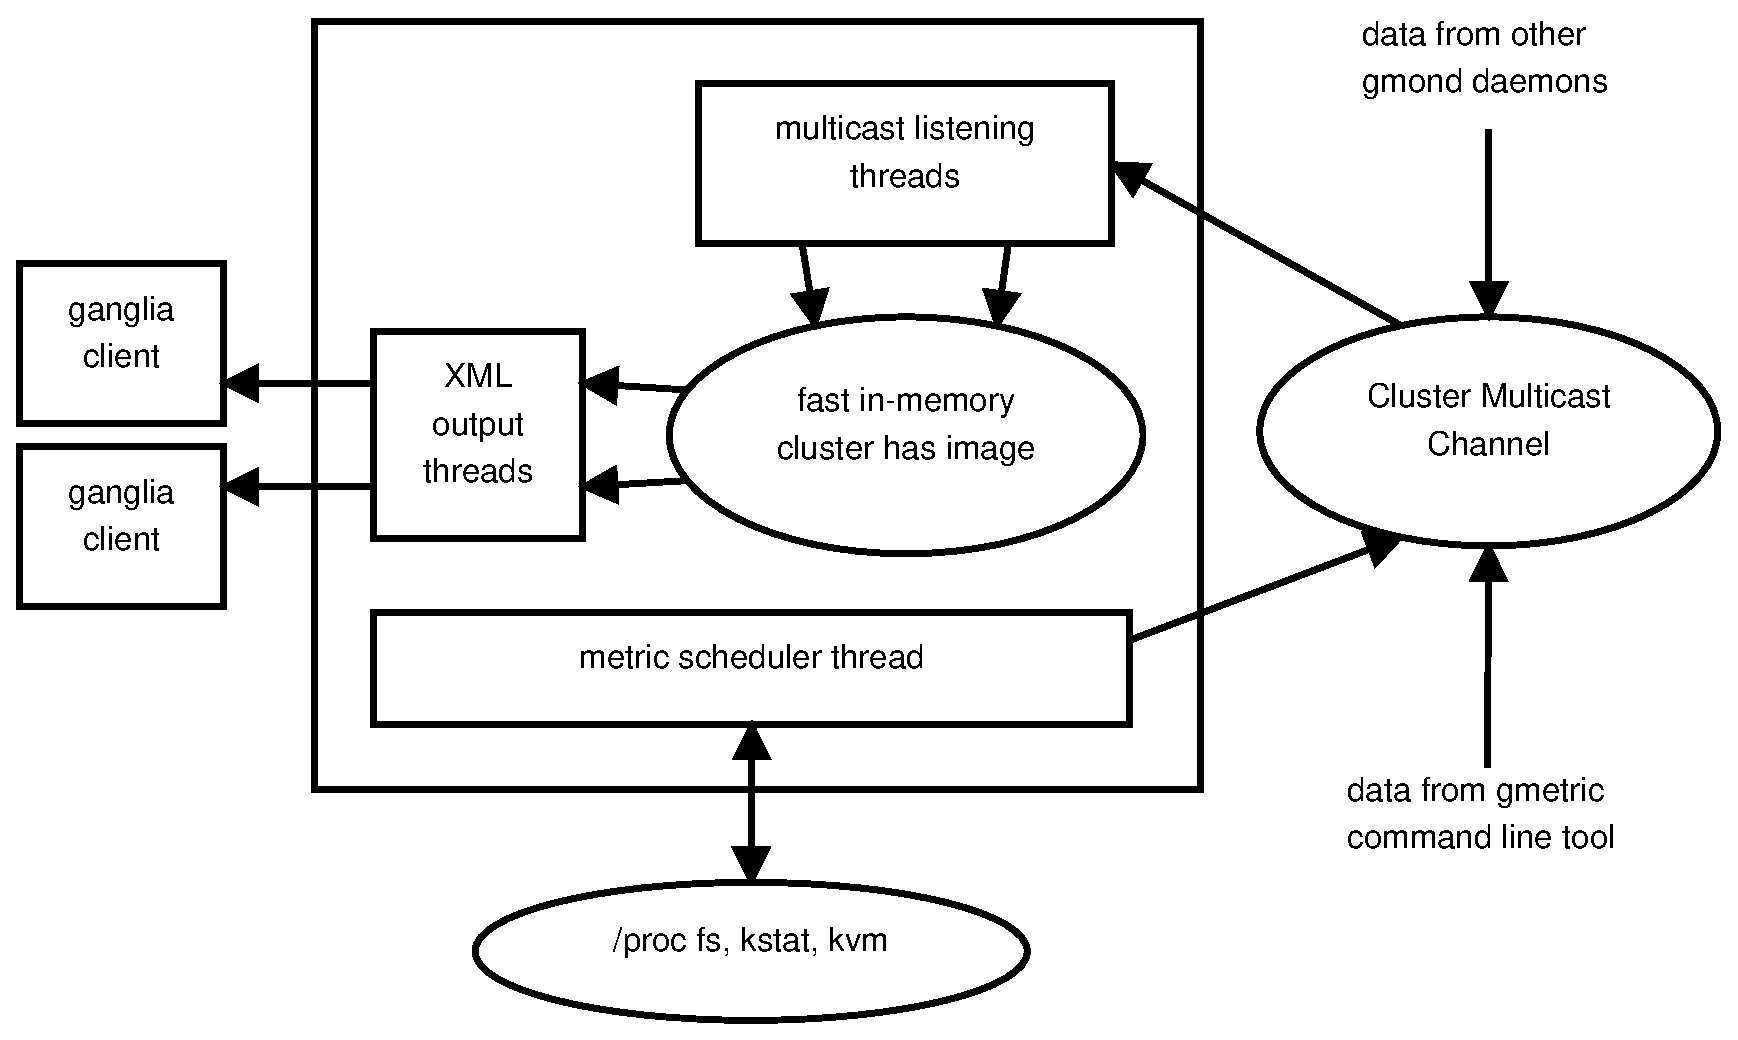
\includegraphics[width=130mm]{images/ganglia.eps}
\caption{Ganglia Data Flow}
\label{figure:ganglia}
\end{figure}

All the data that are gathered from the multicast channel are written to a hash table in memory. The metric data of each node that runs gmond and sends information over the multicast channel are been processed and saved. To send data over the multicast channel, Gmond uses \ac{XDR}. When there is a request over a TCP connection, the response is in XML.

\subsection{Nagios}
Nagios is a monitoring system which provide a scheduler to check hosts and services periodically, and report their status in a \ac{CGI} developed interface. Its large acceptance in industry to monitor service availability has created a large community of developers of custom check commands (plug-ins). It was also accepted from the grid community as the replacement of \ac{SAM} in front of its metrics to periodically parse data from information providers about services availability.

Nagios has a strong back-end, which offers a message bus to integrate with other Nagios installations, to offer the scalability needed to connect site, regional and top level Nagios installations. Information Providers of other Information Services may be customized to be used as Nagios plugins.

Its web based front-end allows the integration with \ac{GOCDB} to handle authentication, using \ac{VOMS} to HTPASSWD system service. Tickets about problems or scheduled downtimes are also handled using Nagios.

Finally, its backend may be scaled-out by using NDOUtils as a service to offer database for the logging of check operations and history. PNP4Nagios is a plug-in that offers visualization of the performance metrics, using the RRDTool. Its distributed monitoring solutions recently were expanded by the \ac{DNX} and the \ac{MNTOS} \cite{Nagios}

\section{European Grid Infrastructure}
Latest \ac{EGI} directive to form regional operation tools forced the use of Nagios \cite{imamagic2007grid} as the main tool of availability \& performance (an so reliability) monitoring of the grid. Each \ac{NGI}/\ac{ROC} (regional level) has its own interface, and hierarchically there is a Super Nagios interface to report the top level view of general system availability. Nagios offers extensions such as NRPE to remotely invoke check commands in inaccessible/private installations. Another important add-on to Nagios is the NdoUtils, which offers an SQL store of history data to the monitoring interface. Nagios Configuration Generator was introduced to help the automatically generation of the configuration based on the information system of nodes and services.

Finally, there has been proposed an integration of \ac{SAM} views to a Nagios customized interface, to offer the last good known \ac{SAM} interface to the old users. Nagios also integrates with \ac{GGUS}, a ticketing system that european grid initiative uses. Monitoring infrastructure in EGI is fully distributed using regional Nagios servers and the corresponding regional MyEGI portals.

\subsection{UK Initiatives}
Brunel University takes part in regional and european initiatives. 5 different \acp{CE} exist, and 3 \acp{SE}, consisting the UKI-LT2-Brunel site. LT2 stands for London Grid, a co-operation with other London Universities. \ac{GridPP} and \ac{NGS} are two collaboration groups that Brunel University is member of.

In \ac{GridPP}, regional monitoring tools exist to provide distributed monitoring services in UK. Regional Nagios and MyEGI/MyEGEE instances co-exist in Oxford University that offer service availability monitoring for all UK sites. Ganglia installations exist in site level deployments, and a Ganglia frontend which aggregates Tier-1 sites is offered through \ac{RAL}.
